\section{Einführung}
\label{sec:chapterexample}

\subsection{Problemstellung}
\label{sec:chapterexample}

Heutzutage liefern diverse Hersteller verschiedene Lösungen für das Türglockensystem. Diese sind meistens Komplettsysteme, die nicht nur das einfache Klingel ermöglichen, sondern auch Zusatzfunktionen wie das Videostreaming anbieten. Diese Systeme sind aber meistens proprietär und werden für sehr hohe Preise verkauft.
\\
Die Komponenten, die für solche Systeme notwendig sind, sind aber heutzutage kostengünstig auf dem Markt erhältlich. Das Erarbeiten preiswerter Lösungen müsste somit möglich sein. 
\\
Natürlich spielen die Kosten einer Türsprechanlage auf die Investitionen eines Neubaus keine grosse Rolle. Sicher besteht aber in diesem Bereich eine Marktlücke und somit die Möglichkeit neue, bessere und günstigere Lösungen zu entwickeln.  

\subsection{Grundidee}
\label{sec:grundidee}

Die Grundidee dieser Arbeit ist es, durch das Zusammenspiel verschiedener Systemen/Technologien, eine kostengünstige und funktionale Türsprechanlage zu entwickeln.
\\ 
Um den Kostenfaktor zu berücksichtigen, soll die Anlage auf schon vorhandene Technologie/Hardware basieren. Somit fallen die hohen Kosten für die Beschaffung proprietärer Hardware weg.
\\
In der Zeit, in der die Hausautomation und das «Internet of things» immer mehr Bedeutung gewinnen, soll die Türsprechanlage diese Standards in Betracht ziehen.   
Dieses System soll den Benutzern ermöglichen, Ihre Sprechtüranlage durch herkömmliche Smartphone oder Tablet zu bedienen.
\\
Klingelt ein Besucher an der Eingangstüre, soll der Wohnungsbesitzer über sein Smartphone darauf aufmerksam gemacht werden. Über eine am Eingang installierte Kamera, bekommt er auch die Möglichkeit den Besucher im Streaming zu sehen und die Türe, falls erwünscht, durch einen Handybefehl zu öffnen.

\subsection{Lösungskonzept}
\label{sec:lösungskonzept}
Die \cref{fig:hwoverview} bietet ein Überblick über den verschiedenen Komponenten die für den Türsprechanlage notwendig sind. Bei der Vorführung werden die Türöffner und die Glocken durch LEDs simulieret. 
An diese Stellen werden zwei Begriffe erklärt die in diesem Dokument von grosse Bedeutung sind. Die erte ist die Türsprechanlage, damit gemeint ist die Gesamtheit der Komponenten die denn Zusammen den Endprodukt darstellen.
Die zweite Begriff ist die Aussensprechstelle. Wie in der \cref{fig:hwoverview} ersichtilich ist in Grunde genommen ein Mikrocontroller mit verschiedene Modulen die an den Eingangstüre installiert wird. Räumlich von der Aussensprechstelle getrennt befindet sich der Server. Diese besteht aus ein Microcontroller die als Server im Einsatz ist, ein Switch die dazu dient die Aussenssprechstelle mit Strom und Datenverbindung zu versorgen und die Relais die den Türöffner und Glocken betätigen.

\begin{figure}[htb!]
	\begin{center}
		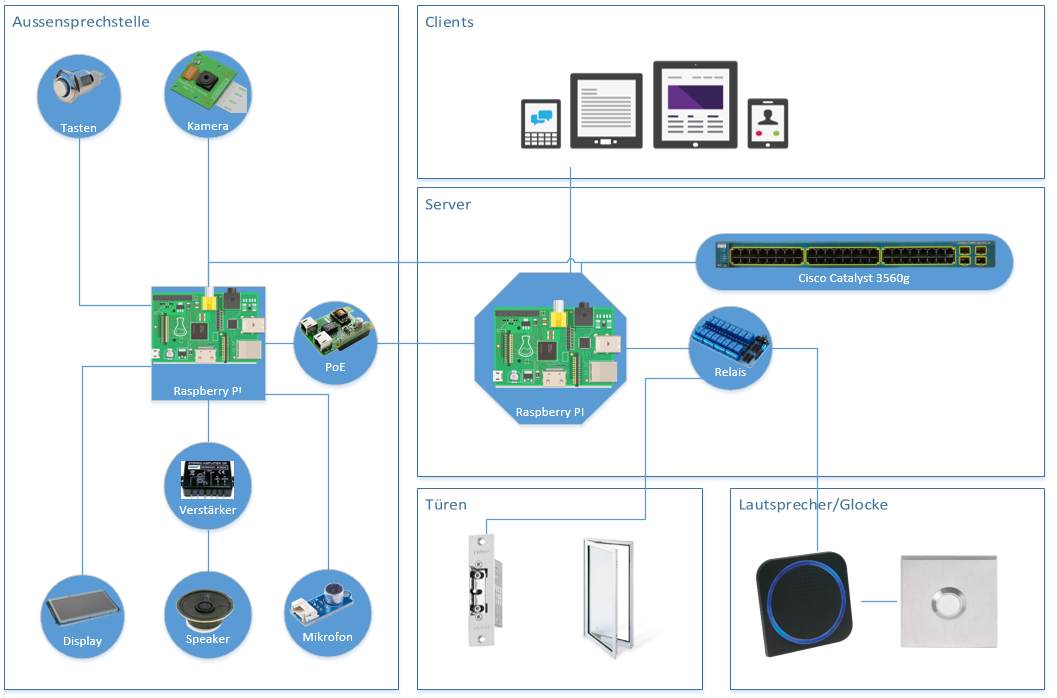
\includegraphics[width=1\textwidth]{hwoverview}
		\caption[Hardware Ecosystem]{Hardware Ecosystem}
		\label{fig:hwoverview}
	\end{center}
\end{figure}
 
\newpage
